%%%%%%%%
\section{Le corium en fond de cuve: est-ce si simple?}
\Intercalaire{Le corium en fond de cuve: est-ce si simple?}
\Titre{Le corium en fond de cuve: est-ce si simple?}
\begin{frame}[fragile]
Pas tout à fait...
\begin{itemize}
\item En premier lieu car \emph{$\left(U_y,Zr_{1-y}\right)O_{2-x}+\left(Fe, \dots\right) \ne$ système ``inerte''} \\
$\rightarrow$ transfert de masse inter-couche et \emph{changement de stratification} en particulier
\item Ainsi, une \emph{évaluation stationnaire} du comportement du corium en cuve \emph{ne suffit pas} ... \emph{ça se complique} \danger
\vskip -0.5\baselineskip
\begin{figure}[H]
\centering 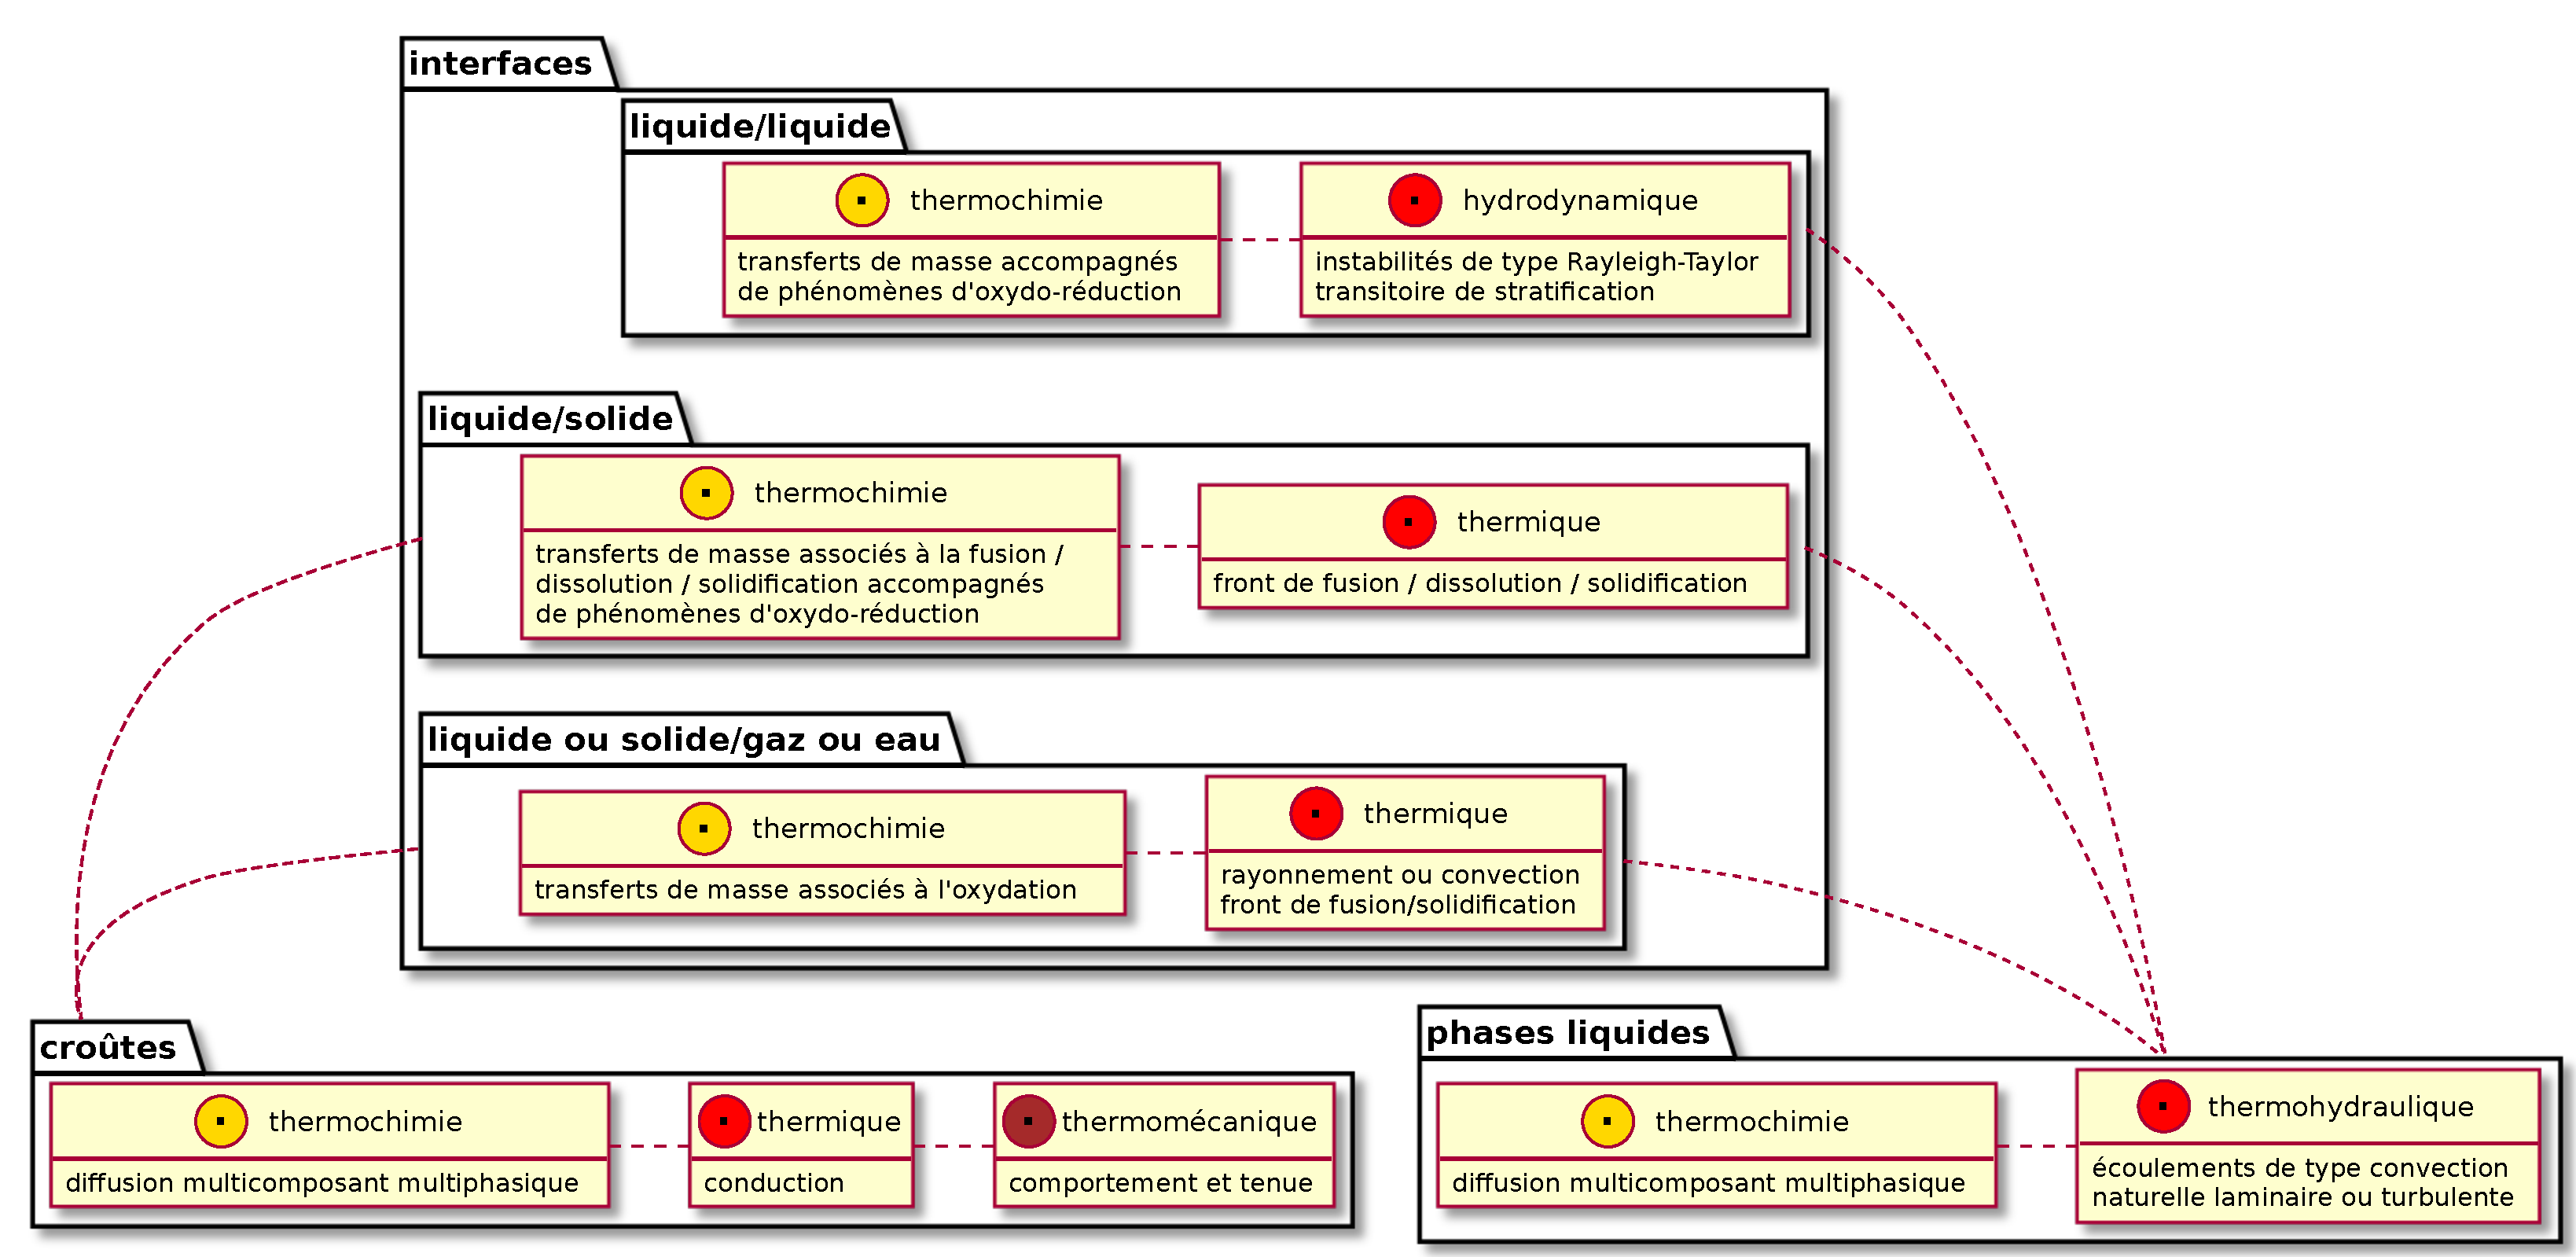
\includegraphics[width=0.7\textwidth]{Figures/corium_en_cuve.pdf}
\vskip -\baselineskip
\caption{\tiny Représentation schématique et partielle de la modélisation du bain de corium en cuve}
\end{figure}
\vskip -0.5\baselineskip
Mais avant de parler de ``thermochimie'', revenons d'abord au \emph{comportement thermohydraulique de la couche mince} et intéressons nous au cas d'une \emph{épaisseur faible} (transitoirement)
\end{itemize}
\end{frame}

%%%%%%%%
\subsection{Thermohydraulique d'une couche métallique supérieure mince}
\begin{frame}[fragile]
\begin{itemize}
\item \emph{Bilan thermique intégral} tel qu'evalué au cours du TD
\begin{columns}[T]
    \begin{column}{0.25\textwidth}
\begin{figure}[H]
\centering 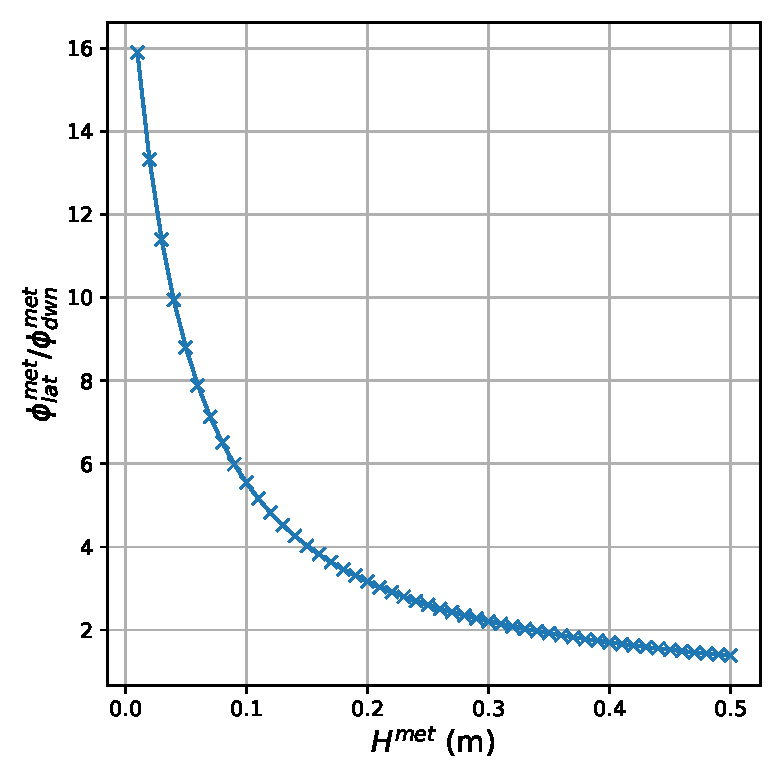
\includegraphics[width=\textwidth]{Figures/Varying_Hmet_2.eps} \\
{\tiny Concentration de flux vs. hauteur de la couche métal (\textit{cf.} TD)}
\end{figure}
    \end{column}
    \begin{column}{0.75\textwidth}
\begin{itemize}
\item Corrélations ``standards'' $\rightarrow$ $\phi^{met}_{lat}/\phi^{met}_{dwn} \nearrow$ lorsque $H^{met} \searrow$ jusqu'à des valeurs très faibles ($<1cm$).
\item Les essais de la campagne BALI-Metal suggère que ces \emph{corrélations surestiment $\phi^{met}_{lat}/\phi^{met}_{dwn}$ pour $H^{met} \le 10$cm}
\item Hormis dans le cas singulier d'une condition adiabatique en surface haute, on s'attend à ce que $\phi^{met}_{lat}/\phi^{met}_{dwn} \rightarrow 0$ quand $H^{met} \rightarrow 0$
\item \emph{Validité de ces corrélations pour cette configuration ?}
\end{itemize}
    \end{column}
\end{columns}
%\item Mais au fait, la surface haute est libre (en l'absence d'oxydation) $\rightarrow$ \emph{quel impact de la déformation de la frontière haute ?}
\item Une question abordée très récemment dans le cadre du projet de recherche européen 
\includegraphics[width=1cm]{Figures/Logo_IVMR.pdf} ~(2015-2019) $\rightarrow$ \emph{illustration de la R\&D menée au CEA}
\end{itemize}
\end{frame}
\subsubsection{Conditions thermiques en limite haute : transfert radiatif et température inhomogène}
\Titre{Couche métallique supérieure - transfert radiatif en surface haute}
\begin{frame}[fragile]
\begin{itemize}
\item Sans le dire, en assimilant le transfert de chaleur vers le haut à celui d'une cavité de Rayleigh-Bénard, on a considéré : \\
\emph{condition inhomogène de transfert radiatif} $\Leftrightarrow$ condition uniforme $T_{up}^{met}$ imposée telle que $\phi_{up}^{BC}\left[T_{up}^{met}\right] = \phi_{up}^{met}\left[T^{met}-T_{up}^{met}\right]$ avec $\phi^{BC}_{up}\left[T^{met}_{up}\right]=\varepsilon_{up}\sigma\left(\left(T^{met}_{up}\right)^4-\left(T^{BC}\right)^4\right)$
\item \emph{Impact de l'inhomogénéité de la condition en limite haute ?}
\item \emph{Etude} paramétrique par \emph{simulations CFD} (code libre 
\includegraphics[width=1cm]{Figures/Logo_TrioCFD.eps} développé au CEA) sur la géometrie parallépipédique des essais BALI-Metal (voir \cite{Peybernes2020})
\begin{itemize}
\item En limite haute, $T_{up}^{met}$ uniforme imposée ou bien condition radiative (locale)
\item $H^{met} \in [1, 10]cm$
\end{itemize}
\begin{columns}[T]
    \begin{column}{0.7\textwidth}
\begin{figure}[H]
\centering 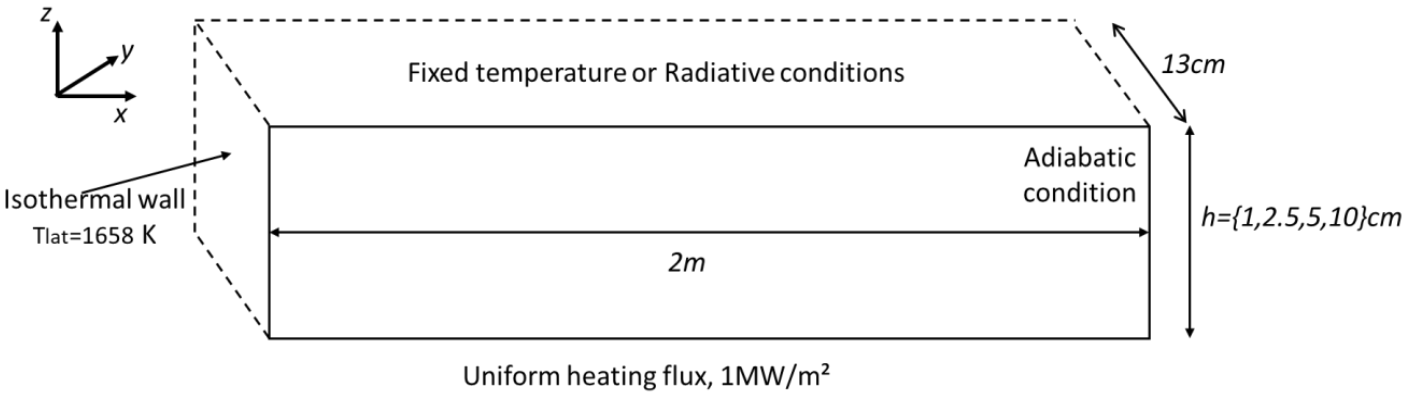
\includegraphics[width=\textwidth]{Figures/Fig3_Peybernes2020.png} \\
{\tiny Domaine de calcul et conditions aux limites des calculs CFD}
\end{figure}
    \end{column}
    \begin{column}{0.3\textwidth}
\begin{figure}[H]
\centering 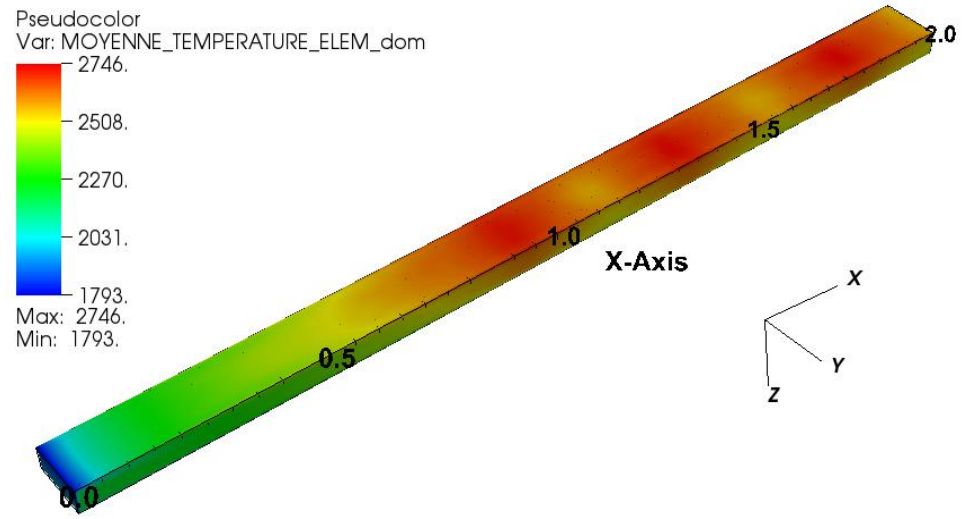
\includegraphics[width=\textwidth]{Figures/Fig5_Peybernes2020.png} \\
{\tiny Température pour $H^{met}=5cm$ (moyennée en temps en régime pseudo-stationnaire)}
\end{figure}
    \end{column}
    \end{columns}
\end{itemize}
\end{frame}
\begin{frame}[fragile]
\vskip -\baselineskip
\begin{columns}[T]
    \begin{column}{0.5\textwidth}
\begin{itemize}
\item \emph{\scriptsize Rôle prédominant de la CL pour $H^{met}$ faible}
\end{itemize}
\vskip -\baselineskip
\begin{figure}[H]
\centering 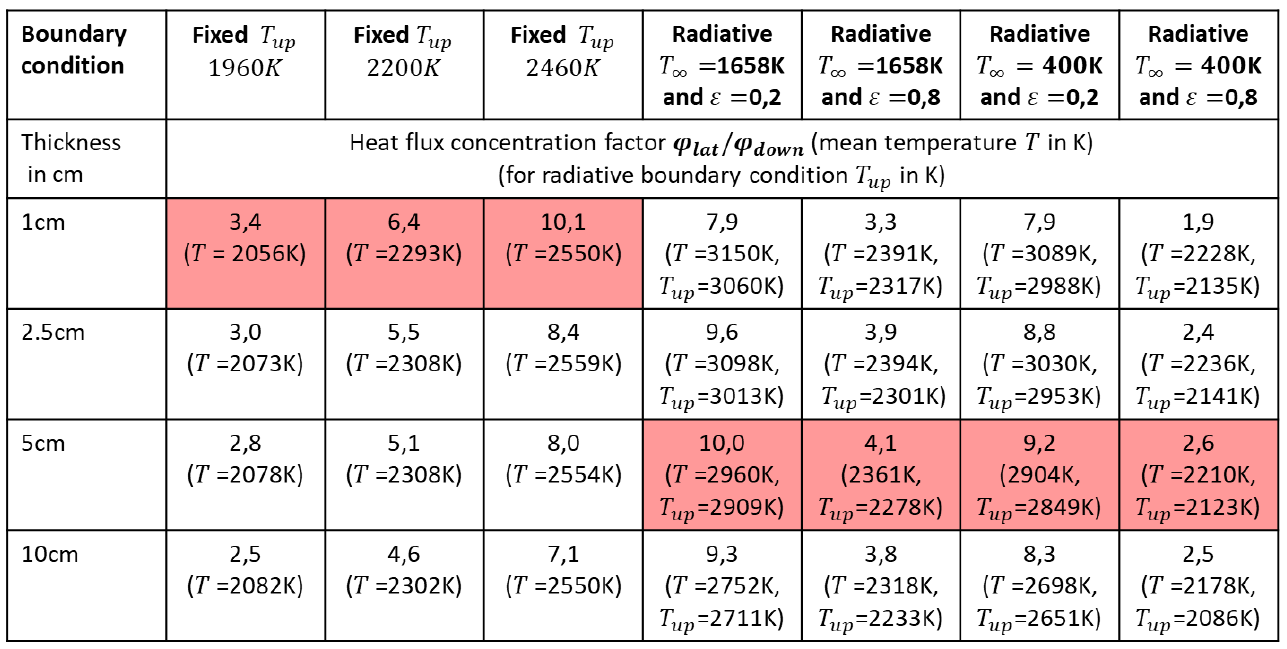
\includegraphics[width=\textwidth]{Figures/TabII_Peybernes2020.png} \\
\vskip -0.5\baselineskip
{\tiny $\phi^{met}_{lat}/\phi^{met}_{dwn}$ fonction de $H^{met}$ et de la condition en limite haute}
\end{figure}
    \end{column}
    \begin{column}{0.5\textwidth}
\vskip -0.8\baselineskip
\begin{figure}[H]
\centering 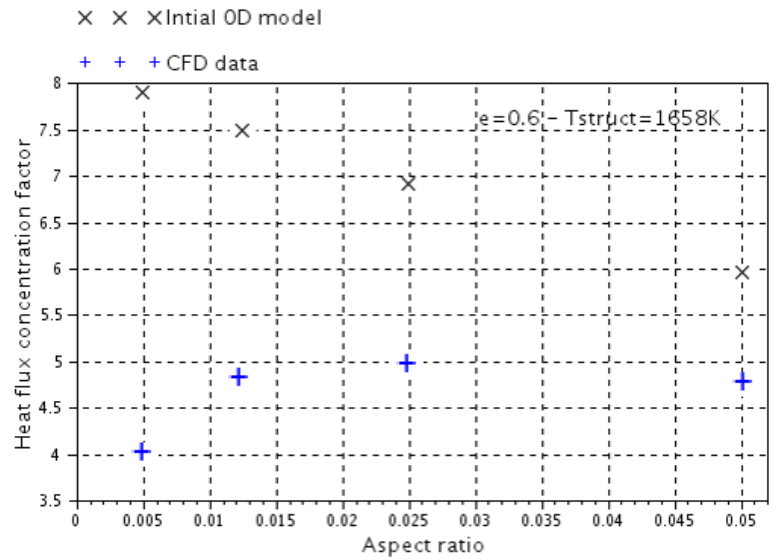
\includegraphics[width=\textwidth]{Figures/Fig6_Peybernes2020.png} \\
\vskip -0.5\baselineskip
{\tiny $\phi^{met}_{lat}/\phi^{met}_{dwn}$ dans le cas $\varepsilon_{up}=0.6$ et $T^{BC}=1658$K}
\end{figure}
    \end{column}
    \end{columns}
\begin{columns}[T]
    \begin{column}{0.6\textwidth}
\begin{figure}[H]
\centering 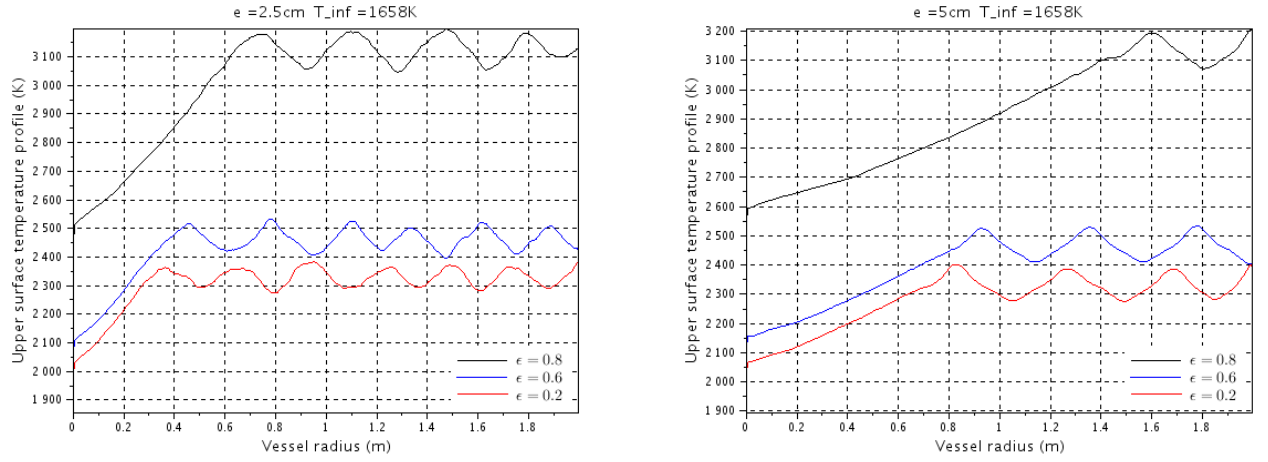
\includegraphics[width=\textwidth]{Figures/Fig8_Peybernes2020.png} \\
\vskip -0.5\baselineskip
{\tiny Profil radiaux de température pour $H^{met}=2.5$cm et $H^{met}=5$cm}
\end{figure}
    \end{column}
    \begin{column}{0.4\textwidth}
\vskip \baselineskip
\begin{itemize}
\item {\scriptsize \emph{Deux nombres adimensionnels} en plus avec \emph{condition radiative}} \\
{\scriptsize e.g. \emph{nombres de Stefan} ($=Pe/Th$) $St \equiv \frac{\varepsilon\sigma T H}{\lambda}$}
\item {\scriptsize Nouvelle corrélation} \\ {\scriptsize $Nu_{up} =  a \times Ra^b Pr^c St_1^d \left(1 + e St_2^f \right)$}
\end{itemize}
    \end{column}
    \end{columns}
\end{frame}
% \subsubsection{Conditions mécaniques en limite haute : Instabilité de Bénard-Marangoni}
% \Titre{Couche métallique supérieure - instabilité de Bénard-Marangoni}
% \begin{frame}[fragile]
% \begin{itemize}
%   \item Frontière supérieure (en l'absence d'oxydation) : une \emph{surface libre déformable}
%   \item Si la \emph{tension de surface $\sigma=f(T)$}, un impact direct sur la thermohydraulique de la couche $\rightarrow$ \emph{effet Marangoni}
%   \item Considérons à nouveau uniquement l'\emph{échange axial} (Rayleigh-Bénard) :
% \begin{columns}[T]
%     \begin{column}{0.35\textwidth}
%     \vskip -\baselineskip
% \begin{figure}[H]
% \centering 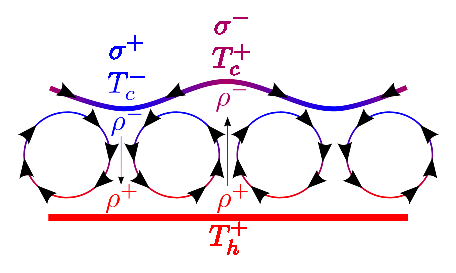
\includegraphics[width=\textwidth]{Figures/RB_BM.eps} \\
%     \vskip -0.5\baselineskip
% {\tiny $\gamma > 0 \rightarrow$ la convection est renforcée}
% \end{figure}
%     \end{column}
%     \begin{column}{0.65\textwidth}
% \begin{itemize}
% \item linéarisation {\scriptsize $\sigma(T) =\sigma_0 - \gamma \left(T-T_0\right)$} avec \emph{$\gamma=-\frac{d\sigma}{dT}(T_0)$}
% \item \emph{$\gamma > 0 \rightarrow$} écoulement de surface dans le \emph{même sens} que cellules de Rayleigh-Bénard
% \item \emph{$\gamma < 0 \rightarrow$} écoulement de surface dans le \emph{sens opposé} des cellules de Rayleigh-Bénard
% \end{itemize}
%     \end{column}
%     \end{columns}
% \item \emph{Instabilité de Bénard-Marangoni} thermique
% \begin{itemize}
% \item $Ma=\frac{\gamma H \Delta T}{\rho_0 \nu \alpha}=\frac{\text{effets thermocapillaires}}{\text{effets dissipatifs (viscosité et diffusion thermique)}}$
% \item \emph{instabilité conditionnelle} (combinée à Rayleigh-Bénard) : \cite{Nield1964} \\
% $\displaystyle \frac{Ra}{Ra_c} + \frac{Ma}{Ma_c} = 1 + \epsilon(Cr,Ga)$ 
% avec $\left\{\begin{array}{rcl} 
%       Cr&=&\frac{\rho\nu\alpha}{\sigma_0 H} ={\tiny\text{déformation de la surface}} \\ 
%       Ga&=&\frac{gH^3}{\nu^2}=\frac{\text{effets de flottabilité}}{\text{effets visqueux}}\end{array}\right.$
% \end{itemize}
% \emph{\textit{a priori}, effet pouvant être important pour $H$ faible}
% \end{itemize}
% \end{frame}
% \begin{frame}[fragile]
% \begin{itemize}
% \item \emph{Evaluation \textit{a priori} pour la couche métallique} (\textit{cf.} \cite{Saas2017})
% \begin{columns}[T]
%     \begin{column}{0.4\textwidth}
%     \vskip -\baselineskip
% \begin{figure}[H]
% \centering 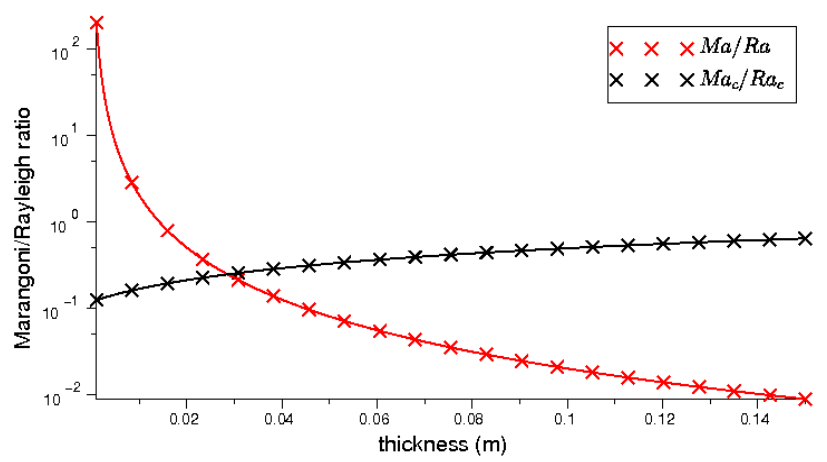
\includegraphics[width=\textwidth]{Figures/Fig3_Saas2017.png} \\
% \end{figure}
%     \end{column}
%     \begin{column}{0.6\textwidth}
%     \vskip -0.5\baselineskip
%     \begin{itemize}
% \item pour $H=0.1$m, en considérant $\Delta T = 100$K et \emph{$\gamma>0$} (fer pur : $4\times 10^{-4}$N.m$^{-1}$.K$^{-1}$), \\
% $Ga\approx 2\times 10^{10}$, $Ra\approx 2\times 10^{7}$, $Ma\approx 5\times 10^{5}$, $Cr\approx 10^{-7}$
% \item \emph{$\frac{Ma}{Ma_c}\ge\frac{Ra}{Ra_c}$ pour $H\le 3$cm}
% \item $Cr\ll 1$ et $Ga\gg 1$: \emph{déformation faible}
% \end{itemize}
%     \end{column}
%     \end{columns}
%     \begin{itemize}
%     \item un effet à prendre en compte \textit{a priori} pour $H \le \sim 5$cm
%     \item simulation simplifée avec une surface plane et une condition limite modifiée : $\cancel{v_x=0} \longrightarrow \frac{\partial v_x}{\partial z} = Ma \frac{\partial T}{\partial x}$
%     \end{itemize}
% \item Mesures de $\sigma(T)$ sur l'installation VITI (CEA Cadarache) \cite{Chikhi2019} : \\ \emph{$\gamma<0$ pour les aciers} 304L (internes cuve) et 16MND5 (paroi cuve)
% \item \emph{Etude} paramétrique par \emph{simulations CFD} (
\includegraphics[width=1cm]{Figures/Logo_TrioCFD.eps}) sur la géometrie parallépipédique des essais BALI-Metal (voir \cite{Peybernes2019})
% \end{itemize}
% \end{frame}
% \begin{frame}[fragile]
% 
% {\footnotesize Quelques résultats extraits de cette étude \cite{Peybernes2019}}
% \begin{columns}[T]
%     \begin{column}{0.6\textwidth}
%     \vskip -\baselineskip
% \begin{figure}[H]
% \centering 
% {\scriptsize $\varepsilon_{up}=0.8$ et $T^{BC}=400$K} \\
% 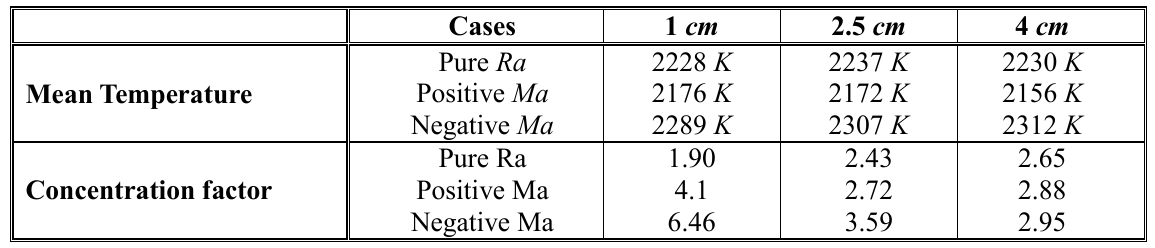
\includegraphics[width=\textwidth]{Figures/TabIV_Peybernes2019.png}
% \end{figure}
%     \end{column}
%     \begin{column}{0.4\textwidth}
%     \begin{itemize}
% \item $T_{(Ra+Ma<0)}>T_{(Ra)}>T_{(Ra+Ma>0)}$
% \item \emph{``Couplage'' fort et non-intuitif avec le refroidissement latéral}
% \end{itemize}
%     \end{column}
%     \end{columns}
% \begin{tabular}{cc}
% \multicolumn{2}{c}{\scriptsize Profil radial de la température de la surface haute ($\varepsilon_{up}=0.2$ et $T^{BC}=1658$K)} \\
% 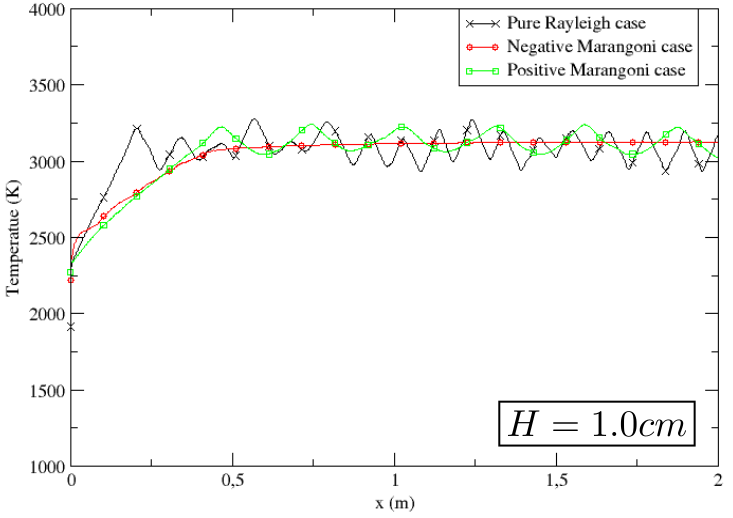
\includegraphics[width=0.35\textwidth]{Figures/Fig5_Peybernes2019.png} & 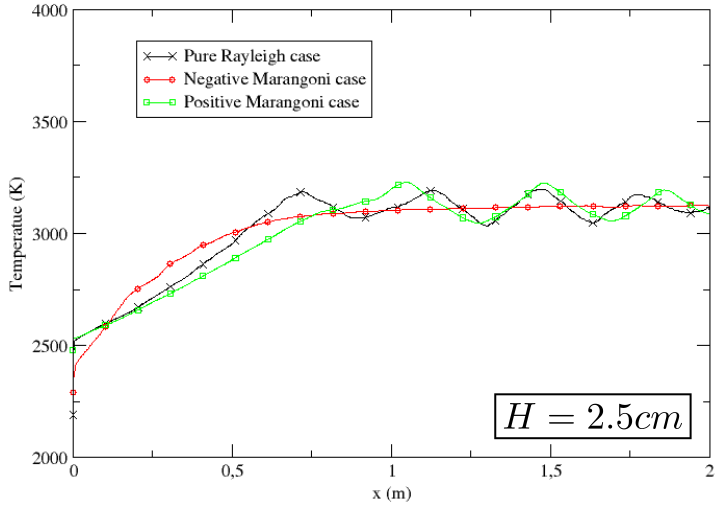
\includegraphics[width=0.35\textwidth]{Figures/Fig6_Peybernes2019.png}
% \end{tabular}
% \begin{itemize}
% \item Loin de la surface latérale, convection ``stoppée'' pour $Ma<0$
% \item Près de la surface latérale, pour $H$ faible, $Ma\lessgtr 0 \rightarrow$ \emph{élargissement de la zone latérale de gradient thermique} $\rightarrow$ refroidissement par transfert radiatif réduit dans cette zone \\
% \emph{Aggravement du focusing effect mais large incertitude} (e.g. $Ma$ solutal, oxydation)
% \end{itemize}
% \end{frame}

%%%%%%%%
\subsection{Corium en cuve et thermochimie}
\Titre{Le corium en fond de cuve: est-ce si simple?}
\begin{frame}[fragile]
Passons maintenant à la \emph{``thermochimie''} {\scriptsize $\left(U_y,Zr_{1-y}\right)O_{2-x}+\left(Fe, \dots\right) \ne$ système ``inerte''}
\begin{figure}[H]
\centering 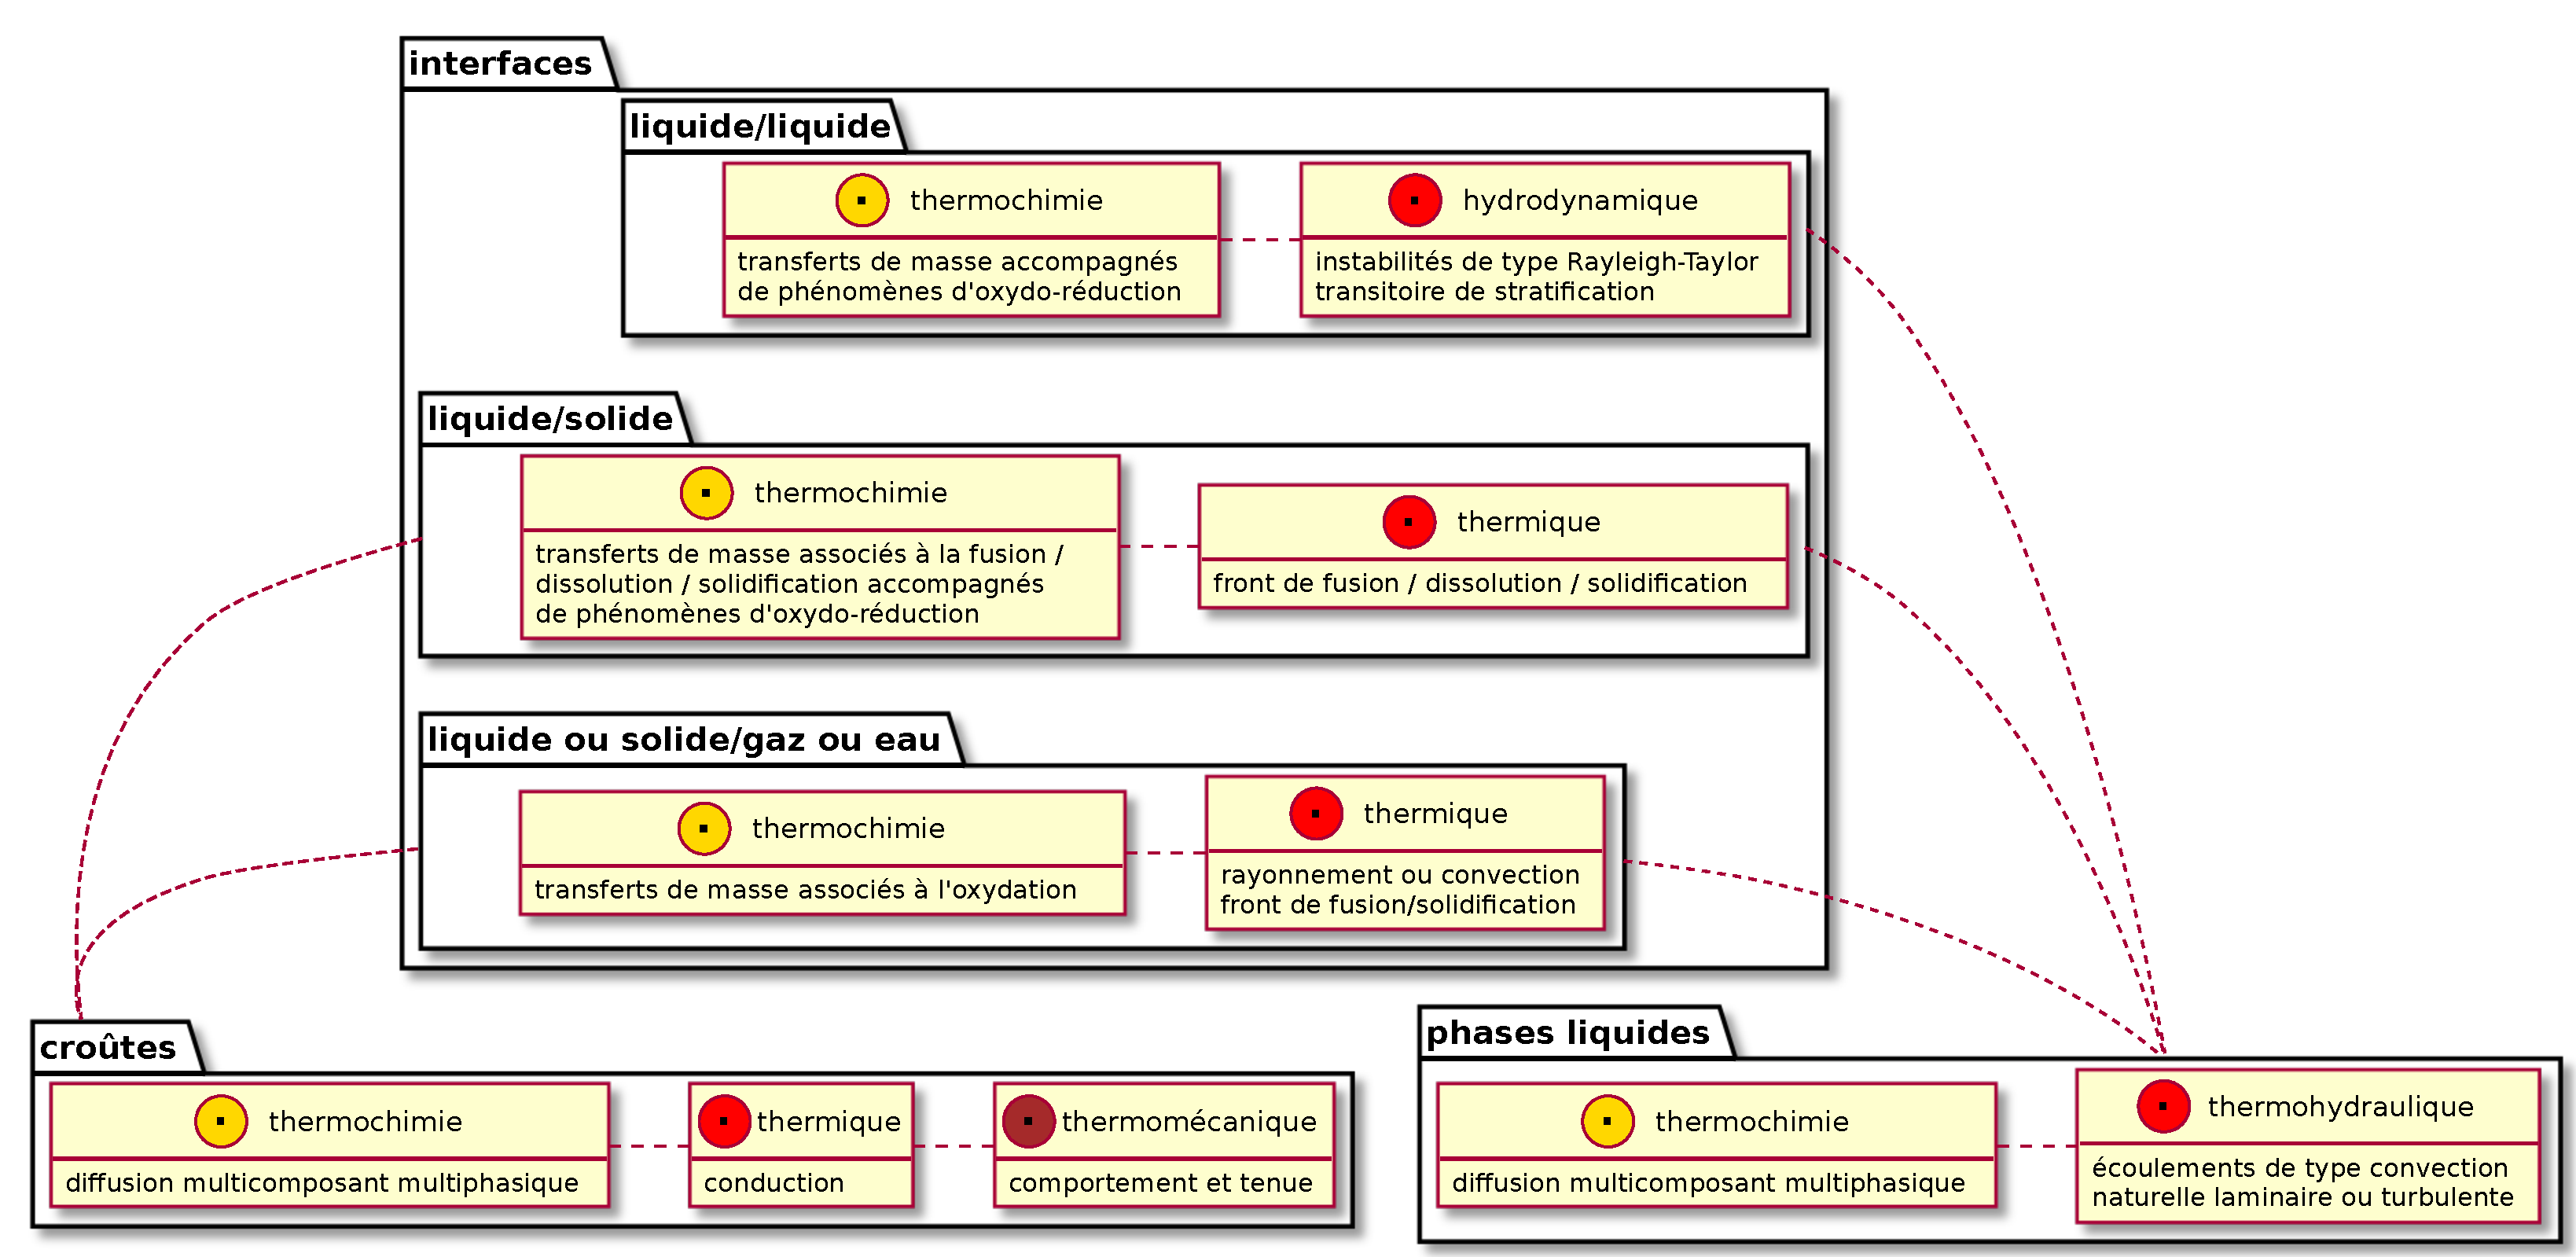
\includegraphics[width=0.75\textwidth]{Figures/corium_en_cuve.pdf}
\vskip -\baselineskip
\caption{\scriptsize Représentation schématique et partielle de la modélisation du bain de corium en cuve}
\end{figure}
\vskip -\baselineskip
\begin{itemize}
\item Nombreux \emph{phénomènes mal connus ou quantifiés}
\item Un phénomène de \emph{premier ordre}, le  \emph{transfert de masse inter-couche} qui, couplé avec l'hydrodynamique, conduit à des \emph{changements de stratification}
\item Présentation de la \emph{phénoménologie} et ouverture sur la \emph{R\&D au CEA} sur ce sujet
\end{itemize}
\end{frame}
\subsection{Stratification des couches liquides}
\Titre{Echanges de masse interfacial et stratification des couches liquides}
\subsubsection{Equilibre thermodynamique de $\left(U_y,Zr_{1-y}\right)O_{2-x}+\left(Fe, \dots\right)$}
\Titre{Equilibre thermodynamique de $\left(U_y,Zr_{1-y}\right)O_{2-x}+\left(Fe, \dots\right)$}
\begin{frame}
      \vskip -0.5\baselineskip
      \begin{itemize}
\item \emph{Lacune de miscibilité} $\rightarrow$ deux liquides à l'\emph{équilibre} ($T$ donnée) avec \emph{$\rho_{met}\lessgtr \rho_{oxy}$} suivant :
\begin{columns}[T]
  \begin{column}{0.45\textwidth}
    \begin{tabularx}{\textwidth}{CCC}
    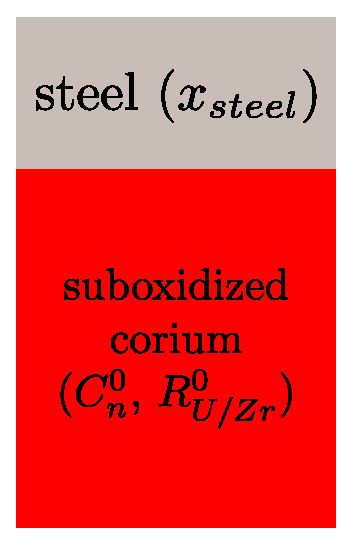
\includegraphics[width=0.2\textwidth]{Figures/schema_stratif_2_ini.eps} & 
    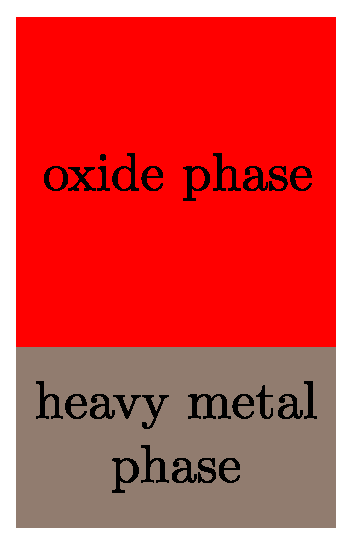
\includegraphics[width=0.2\textwidth]{Figures/schema_stratif_2_hm.eps} &
    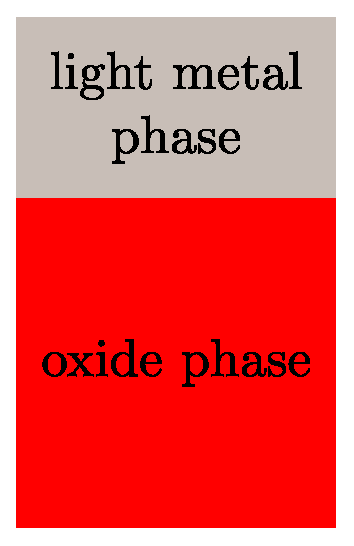
\includegraphics[width=0.2\textwidth]{Figures/schema_stratif_2_lm.eps} \n
    \tiny Etat initial & \tiny Métal ``lourd'' & \tiny Métal ``léger''
    \end{tabularx}
  \end{column}
  \begin{column}{0.6\textwidth} 
  \begin{itemize}
    \item le degré d’oxydation du Zr ($C_n^0$) et du rapport molaire U/Zr ($R_{U/Zr}^0$) du corium oxyde initial
    \item le rapport entre les masses d'acier et de corium oxyde initialement mises en présence ($x_{steel}$)
  \end{itemize}
  \end{column}
\end{columns}
\end{itemize}
\begin{columns}[T]
  \begin{column}{0.4\textwidth}
  \begin{itemize}
    \item \emph{Expériences à ``petite échelle''}
    \item $\diameter \le 7$cm et $m_{oxy}$ $\sim$ 100g à 2kg
    \item e.g. programme MASCA (OCDE) \cite{Tsurikov2007}
  \end{itemize}
  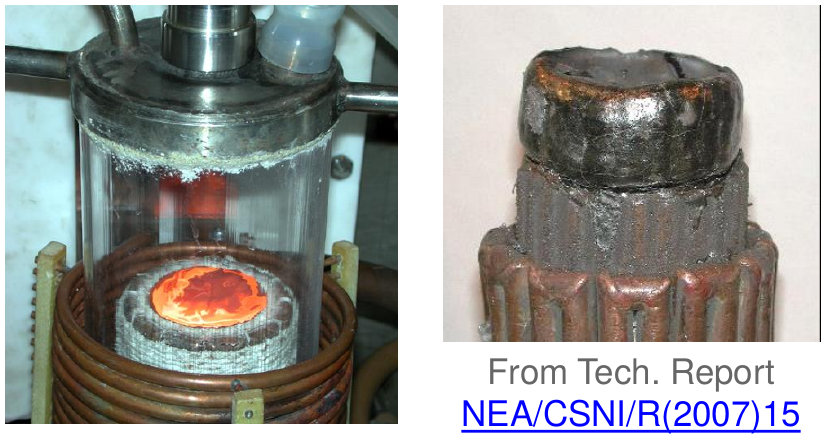
\includegraphics[width=\textwidth]{Figures/rasplav3.png} 
  \end{column}
  \begin{column}{0.6\textwidth} 
\renewcommand{\arraystretch}{0.1}
\centering {\tiny Densités des phases oxyde ($\rho_{oxy}$) et métal ($\rho_{met}$) calculées à l'équilibre}
\begin{tabularx}{\textwidth}{>{\setlength{\baselineskip}{0.5\baselineskip}}C >{\setlength{\baselineskip}{0.5\baselineskip}}C}
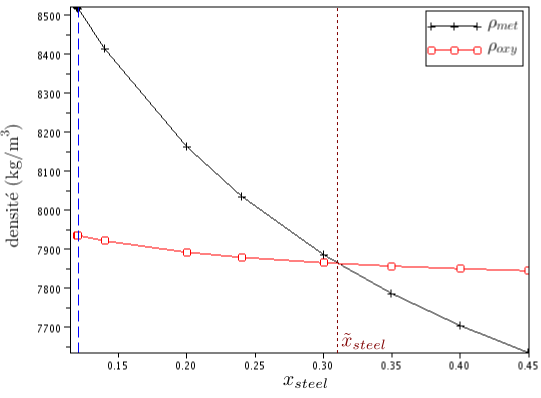
\includegraphics[width=0.48\textwidth]{Figures/densities_vs_x0met_MA3_2840K_new.png} & 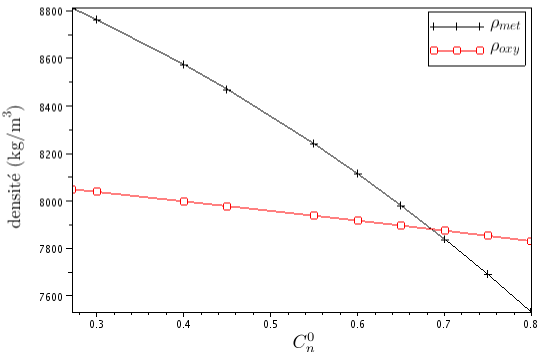
\includegraphics[width=0.48\textwidth]{Figures/densities_vs_Cn_MA9_2855K_new.png} \n
{\tiny En fonction de $x_{steel}$ pour ($\bar{T}=2840$K, $C_n^0=36.5\%$ et $R_{U/Zr}^0=1.14$) $\rightarrow$ MASCA-MA-3} & {\tiny En fonction de $C_n^0$ pour ($\bar{T}=2855$K, $x_{steel}=0.1$ et $R_{U/Zr}^0=1.17$) $\rightarrow$ MASCA-MA-9}
\end{tabularx}
\renewcommand{\arraystretch}{1.0}
      \vskip -0.5\baselineskip
\begin{itemize}
\item Représentation thermodynamique : méthode CALPHAD $\rightarrow$ Energie de Gibbs des phases $\wp$
\item Lois de densité $\rho_{\wp}\left(\text{composition}\right)$
\end{itemize}
  \end{column}
\end{columns}
\end{frame}
\subsubsection{Cinétique de stratification : échange interfacial et instabilité de Rayleigh-Taylor}
\Titre{Cinétique de stratification}
    \begin{frame}
      \vskip -0.5\baselineskip
\begin{columns}[T]
  \begin{column}{0.5\textwidth}
    \begin{tabularx}{\textwidth}{CC}
    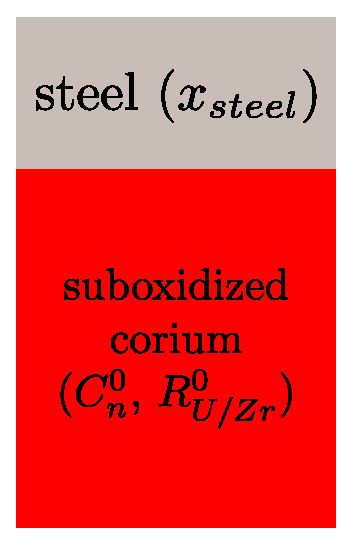
\includegraphics[height=0.25\textheight]{Figures/schema_stratif_2_ini.eps} &
    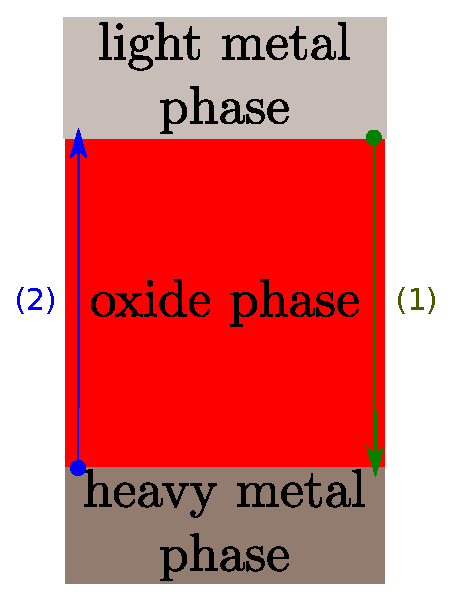
\includegraphics[height=0.30\textheight]{Figures/schema_stratif_3.eps} \n
    \tiny Etat ``initial'' (deux couches) & \tiny Etat transitoire (trois couches)
    \end{tabularx}
  \end{column}
  \begin{column}{0.55\textwidth} 
    \hskip -0.7cm \begin{minipage}{1.1\textwidth}
  \begin{itemize}
\item Transitoire AG en fond de cuve \\ $\rightarrow$ \emph{apport progressif d'acier fondu}
\item \emph{Deux transitoires de stratification} associés à ces équilibres à deux couches potentiels :
\begin{itemize}
\item[\textcolor{OliveGreen}{(1)}] formation de la couche métallique lourde \\
\emph{$\rightarrow$ Aggravement du risque de focusing effect}
\item[\textcolor{blue}{(2)}] retour à une stratification ``normale'' \\
\emph{$\rightarrow$ Remontée de métal ``surchauffé''}
\end{itemize}
  \end{itemize}
\end{minipage}
  \end{column}
\end{columns}
      \begin{itemize}
      \item Ce que l'on peut dire \textit{a priori} des \emph{phénomènes mis en jeu} :
      \begin{itemize}
      \item \emph{transfert de masse interfacial} $\rightarrow$ transitoire \textcolor{OliveGreen}{(1)} : U et Zr vers l’acier \\
      {\tiny (décalage à droite de \ce{ UO_2 + Zr <=> ZrO_2 + U } dans l'oxyde à l’interface)}
      \item transport de masse intra-phase
      \item ``inversion'' de $\rho_{oxy} \lessgtr \rho_{met}$ $\rightarrow$ \emph{instabilité de Rayleigh-Taylor}
      \item mouvement hydrodynamique d'inversion de la position des phases
      \end{itemize}
      \item Deux \emph{cinétiques combinées} : ordres de grandeur pour \textcolor{OliveGreen}{(1)} :
      \begin{itemize}
\item transport de masse intra-phase : $\tau_m = \frac{H^2}{D} \frac{1}{Sh}$ (masse $\Leftrightarrow$ $\tau_h = \frac{H^2}{\alpha} \frac{1}{Nu}$ chaleur) \\
dans le métal, pour $H=5cm$, $Gr\approx4\times 10^{7}$, $Nu\approx10$ (\textit{cf.} TD) \\
en considérant $D=5\times 10^{-9}$m$^2$.s$^{-1}$, $Sh/Nu\approx80$ $\rightarrow$ \emph{$\tau_m \approx 10$min}
\item vitesse terminale de goutte pour l'instabilité de Rayleigh-Taylor $\rightarrow$ \emph{$\sim 10s.m^{-1}$}
      \end{itemize}
      \hskip -0.5cm $\rightarrow$ \emph{Transport intra-phase bien plus lent que mouvement hydrodynamique}
\end{itemize}
    \end{frame}
    \begin{frame}
    
      \emph{\small Observations expérimentales indirectes :}
      \begin{itemize}
      \item Essais à \emph{``petite échelle''} : équilibre atteint en \emph{moins de 20'}, \emph{mouvement ``en bloc''} et très rapide à l'inversion des phases
      \item \emph{Une seule expérience de plus grande échelle} (MASCA-RCW) stoppée au bout de 22' \\ ($\diameter \le 18$cm et $m_{oxy} \approx 45$kg et $x_{steel}\approx 0.1$) - transitoire \textcolor{OliveGreen}{(1)}
      \begin{columns}
\begin{column}{0.65\textwidth}
\vskip 0.5\baselineskip
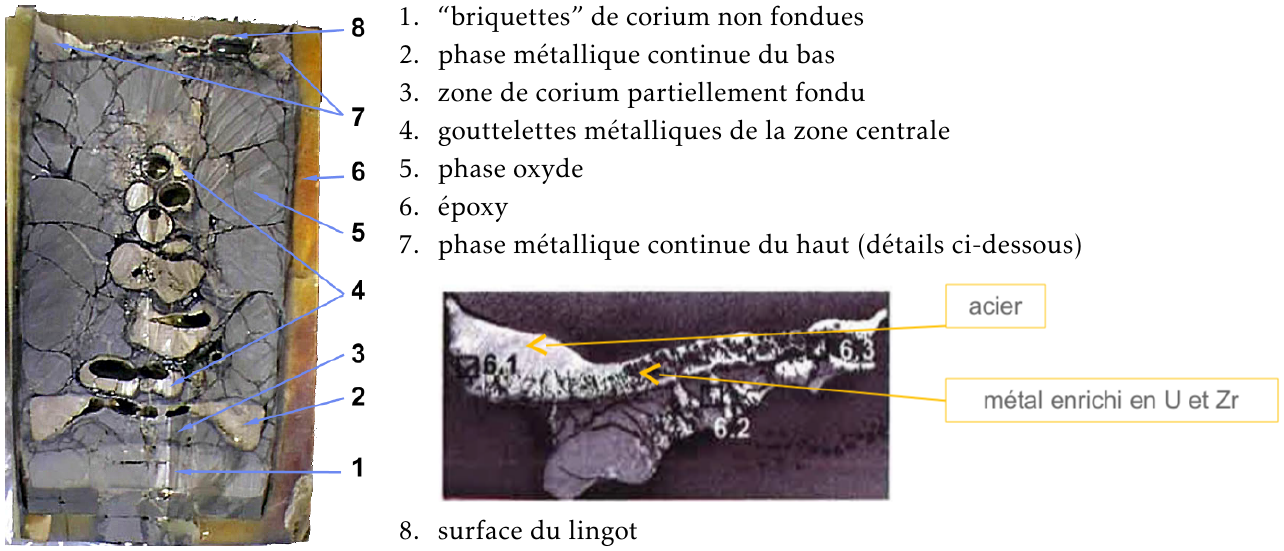
\includegraphics[width=\textwidth]{Figures/rcw.png}
\end{column}
\begin{column}{0.4\textwidth}
\hskip -0.8cm \begin{minipage}{1.1\textwidth}
  \begin{itemize}
\item état final $\sim$ un instant du transitoire de formation de la phase métallique lourde
\item Rayleigh-Taylor en gouttelettes
\item gradient de concentration en U, Zr dans la couche métallique supérieure
\end{itemize}
\end{minipage}
\end{column}
      \end{columns}
      \item \emph{Cinétique limitante : celle du transfert de masse} (transport multicomposant, multiphasique)
      \item Pour les cas réacteurs, évaluation du temps caractéristique : \\ $\sim 1$h pour \textcolor{OliveGreen}{(1)} et plus élevé pour \textcolor{blue}{(2)} ...
\end{itemize}
    \end{frame}
\begin{frame}[fragile]
\begin{itemize}
\item ... Une \emph{incertitude forte} / des modèles (intégraux) en manque de calage/validation
\begin{itemize}
\item MASCA-RCW ne donne qu'un information indirecte sur le transitoire
\item Aucune expérience caractérisant le transitoire \textcolor{blue}{(2)} de retour à une stratification ``normale'' 
\item Impact d'une croûte à l'interface oxyde/acier
\end{itemize}
\item \emph{Important ! $\rightarrow$ meilleure quantification du comportement transitoire du corium en cuve}
\item En particulier, \emph{R\&D au CEA} :
\begin{columns}
 \begin{column}{0.55\textwidth}
\begin{itemize}
\item Modélisation et \emph{simulation ``mésoscopique''} (CFD) \cite{Zanella2020}
\item Caractérisation expérimentale de la \emph{dissolution d'une croûte de corium oxyde par de l'acier fondu} \cite{Pivano2019}
\item Conception d'un \emph{dispositif experimental \\ $\sim$ MASCA-RCW} mais avec \emph{suivi en ligne des interfaces} par mesure acoustique \cite{Cavaro2019}
\end{itemize}
 \end{column}
 \begin{column}{0.1\textwidth}
 \begin{minipage}{\textwidth}
\movie[showcontrols,width=\textwidth,height=0.5\textheight,externalviewer]{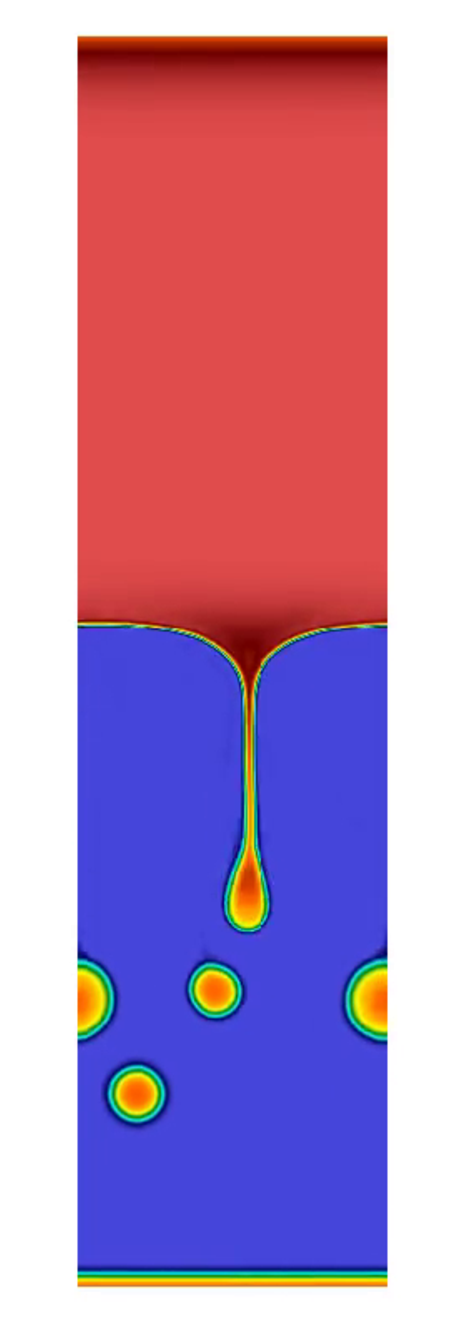
\includegraphics[height=0.5\textheight]{Figures/movie_RT_snapshot.eps}}{Figures/movie_RT.mov}
\end{minipage}
 \end{column}
 \begin{column}{0.35\textwidth}
 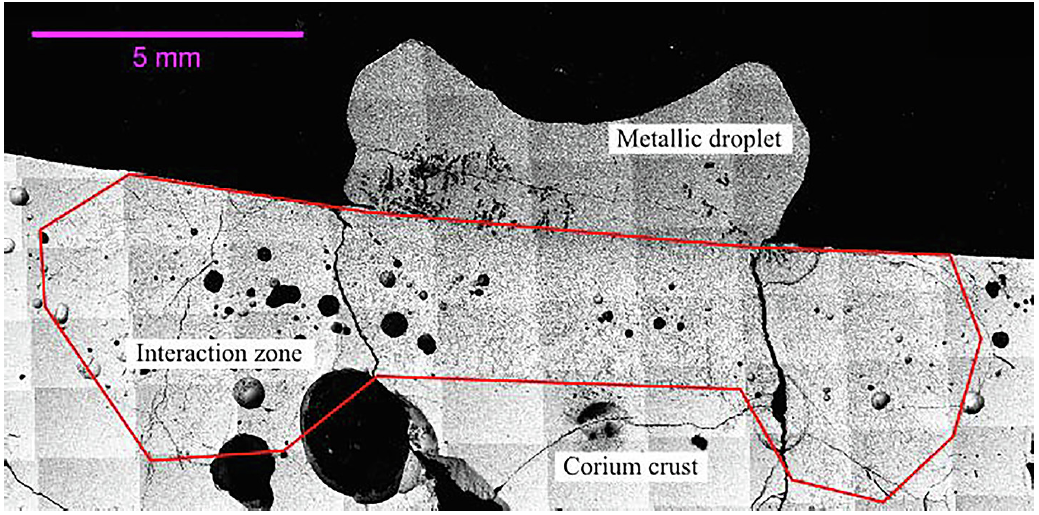
\includegraphics[width=\textwidth]{Figures/cormet.png} \\
 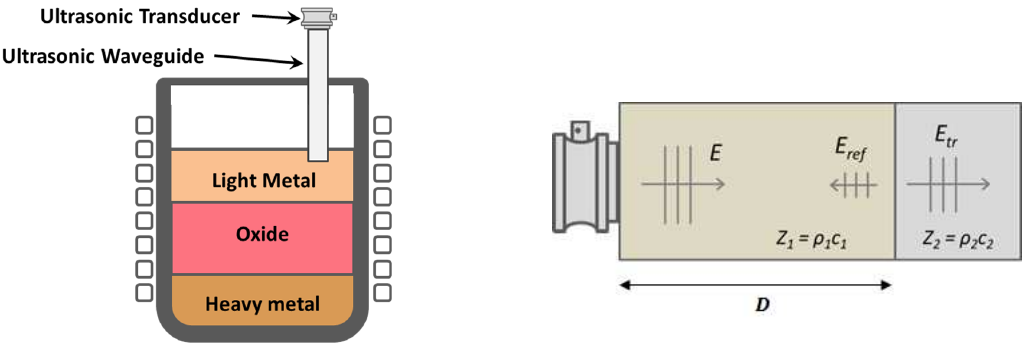
\includegraphics[width=\textwidth]{Figures/stromboli.png}
 \end{column}
\end{columns}
\end{itemize}
\end{frame}
\Intercalaire{Illustration du risque de percement de la cuve en transitoire \\ Résultats de simulation avec le code PROCOR \\ (développé au CEA Cadarache)}
\section{Illustration du risque de percement de la cuve en transitoire}
\Titre{Illustration du risque de percement de la cuve en transitoire : résultats PROCOR}
\begin{frame}[fragile]
\vskip -0.8\baselineskip
\begin{figure}[H]
\centering 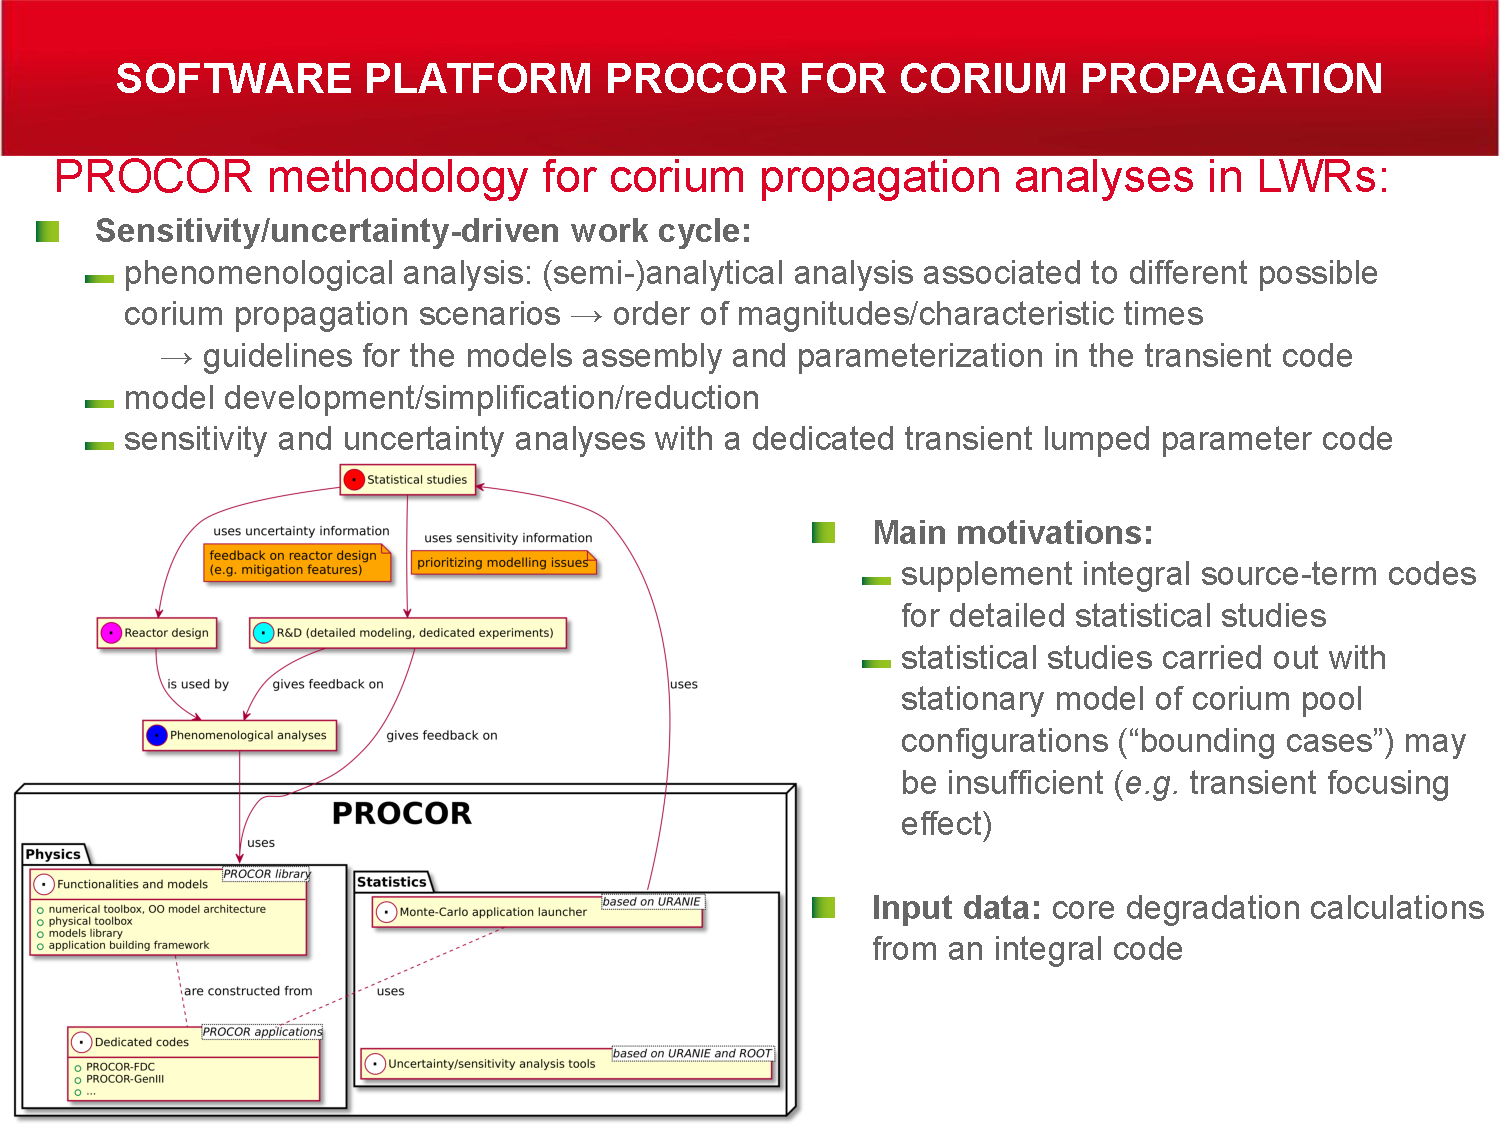
\includegraphics[height=\textheight]{Figures/procor_0a.pdf} 
\end{figure}
\end{frame}
\begin{frame}[fragile]
\vskip -0.8\baselineskip
\begin{figure}[H]
\centering 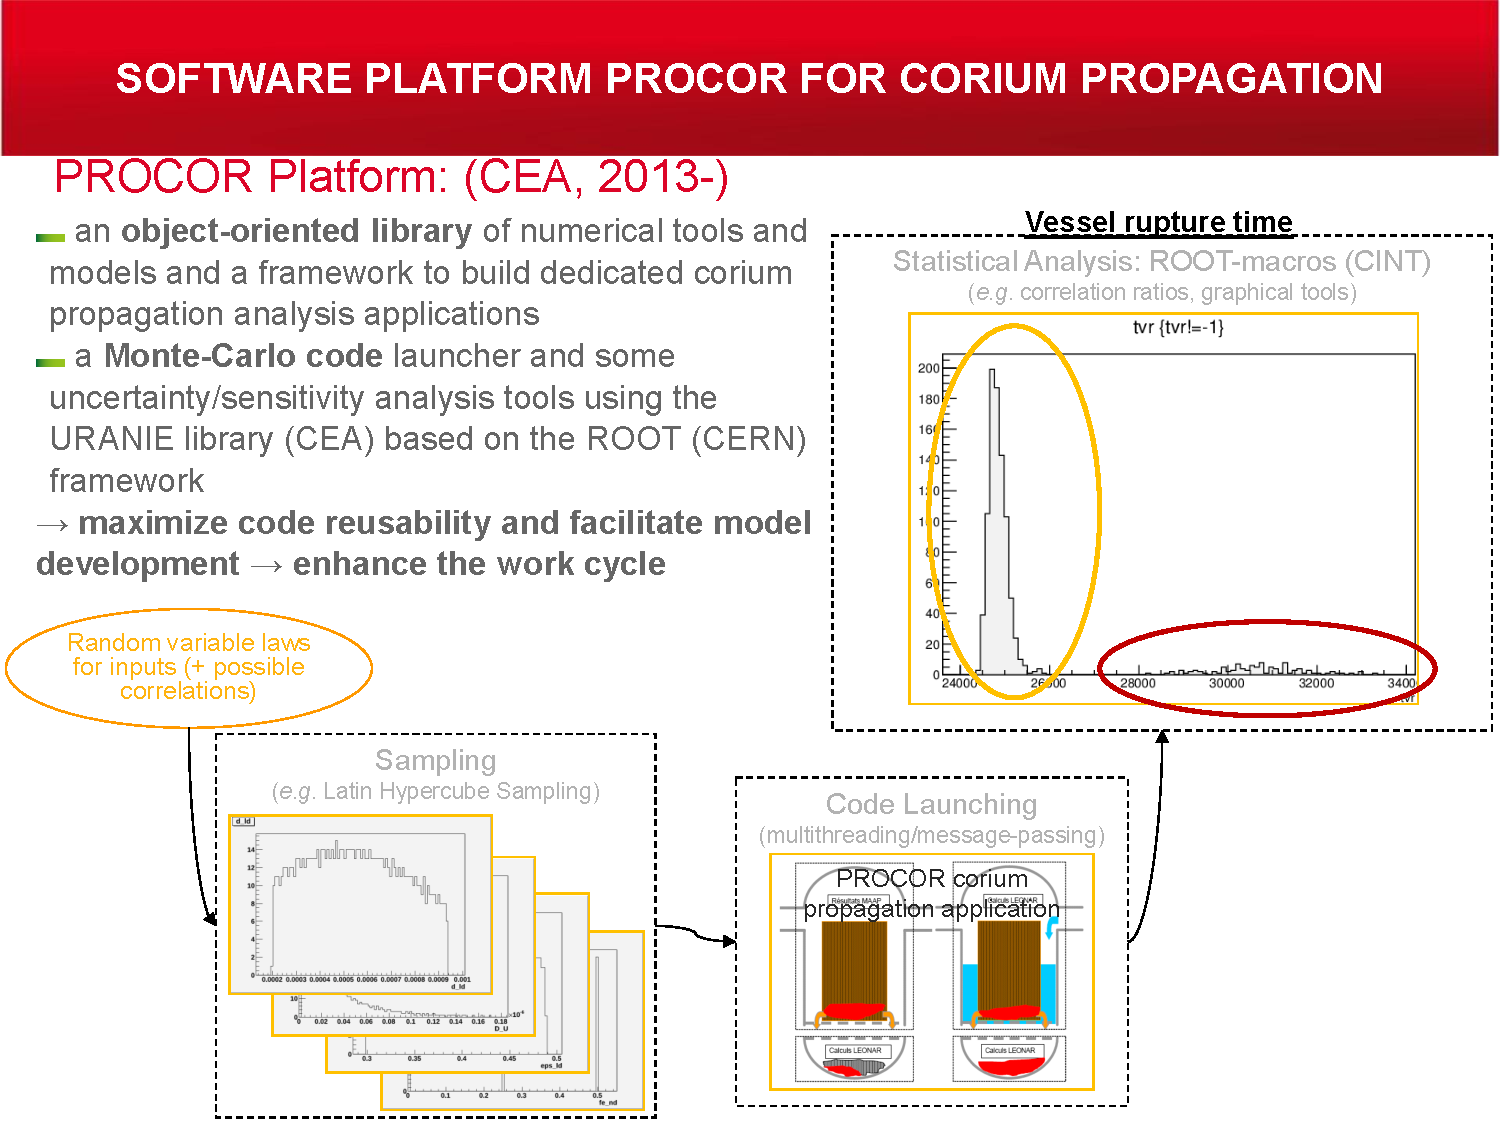
\includegraphics[height=\textheight]{Figures/procor_0b.pdf} 
\end{figure}
\end{frame}
\begin{frame}[fragile]
\vskip -0.8\baselineskip
\begin{figure}[H]
\centering 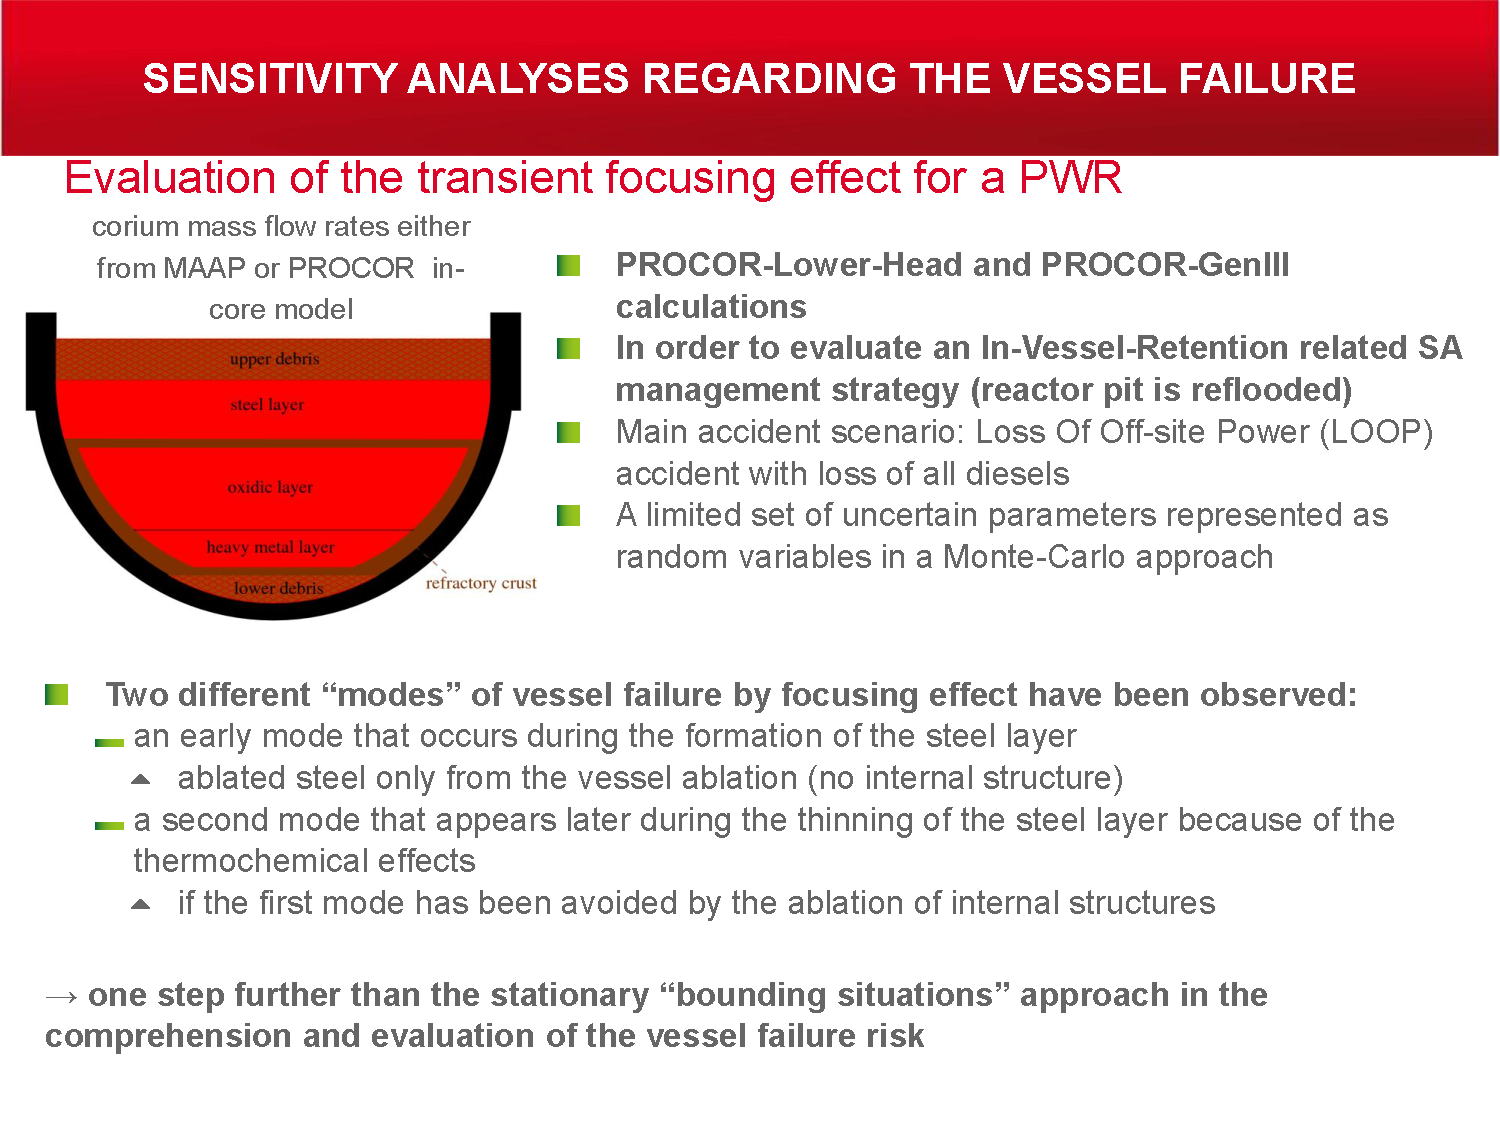
\includegraphics[height=\textheight]{Figures/procor_1.pdf} 
\end{figure}
\end{frame}
\begin{frame}[fragile]
\vskip -0.8\baselineskip
\begin{figure}[H]
\centering 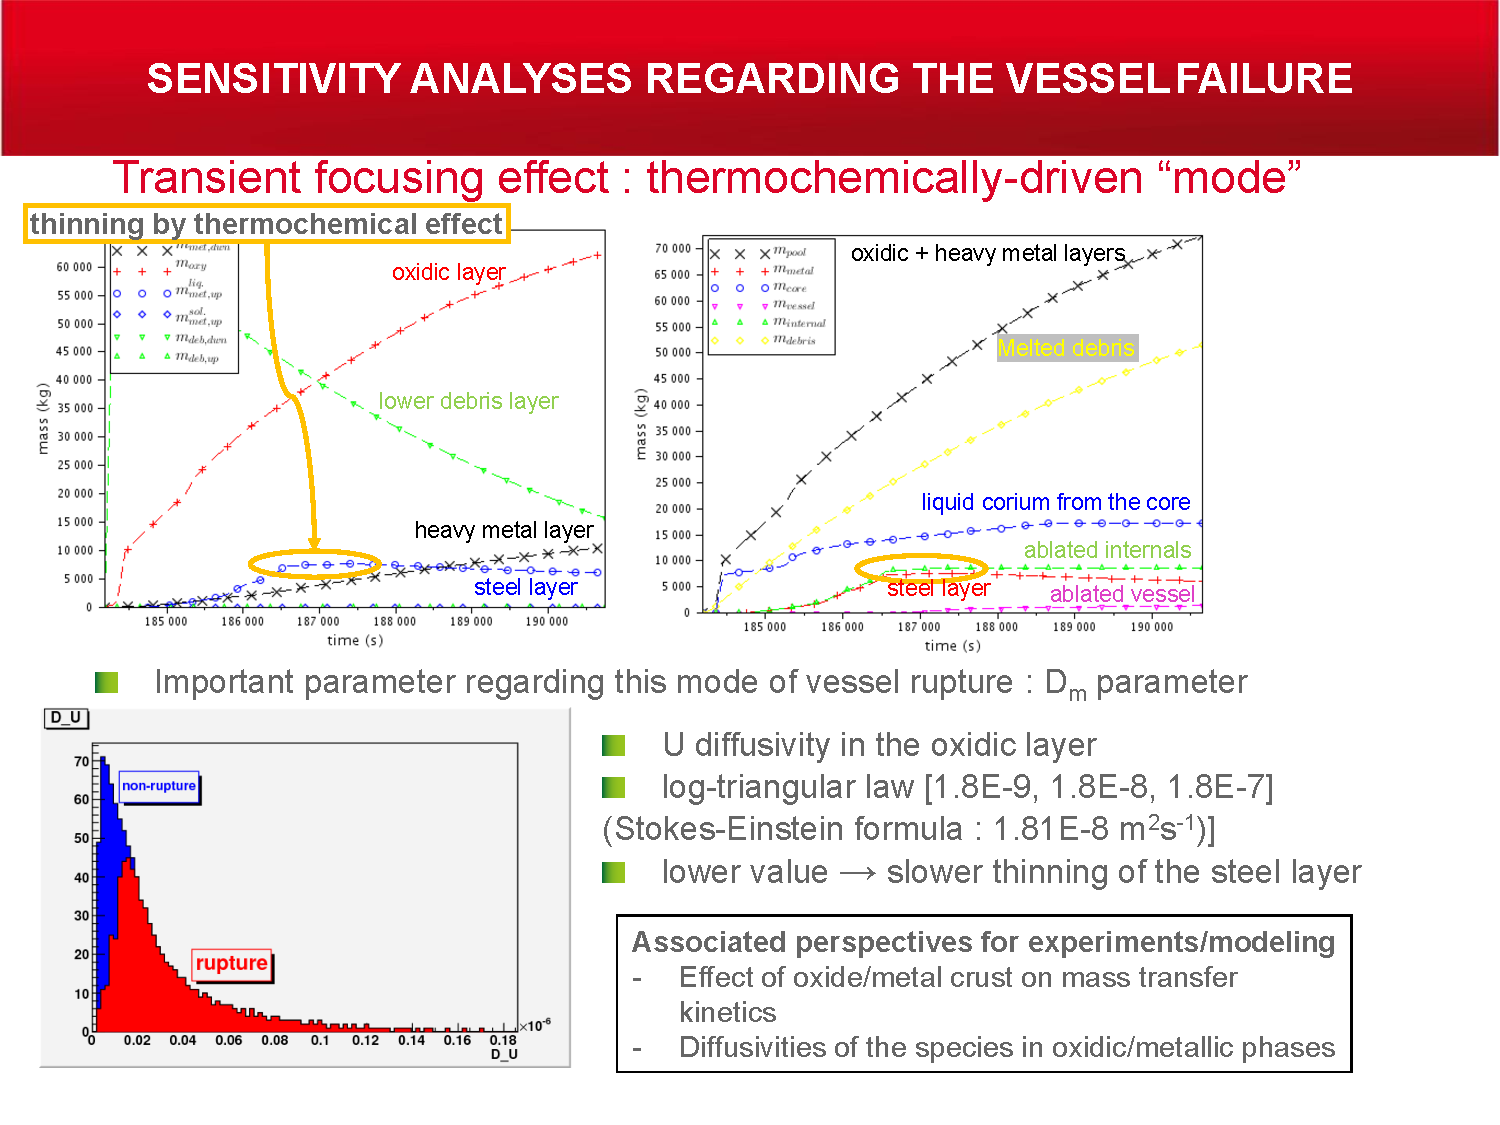
\includegraphics[height=\textheight]{Figures/procor_2.pdf} 
\end{figure}
\end{frame}

%%%%%%%%
\Intercalaire{Introduction au code PROCOR}
\section{Introduction au code PROCOR}
\Titre{Introduction au code PROCOR}
\begin{frame}[fragile]
\end{frame}